\documentclass[abstract=on,10pt,a4paper,bibliography=totocnumbered]{article}
\usepackage[paper=a4paper,left=35mm,right=35mm,top=25mm,bottom=30mm]{geometry}
\usepackage[doublespacing]{setspace}
\usepackage[english]{babel}
\usepackage[utf8]{inputenc}
\usepackage[round]{natbib}
\usepackage{amsmath}
\usepackage{colortbl}
\usepackage{amsfonts}
\usepackage{amssymb}
\usepackage{gensymb}
\usepackage{graphicx}
\usepackage{tikz}
\usepackage{enumerate}
\usepackage{enumitem}
\usepackage{subcaption}
\usepackage{booktabs}
\usepackage[hidelinks]{hyperref}
\usepackage[nameinlink]{cleveref}
% \usepackage{lineno}
\usepackage{multirow}
\usepackage{arydshln}
\usepackage[flushleft]{threeparttable}
\usepackage[nomarkers, nolists]{endfloat}

%------------------------------------------------------------------------------
%	Some Styling
%------------------------------------------------------------------------------
% Creating some TikZ styles
\tikzset{
  nonterminal/.style = {rectangle
    , minimum size = 6mm
    , very thick
    , draw = black!
  }
}

% Changing the style of captions in figures etc.
\captionsetup{labelfont=bf, format=plain, font=small}

% Change how equations are referenced
\renewcommand{\theequation}{Equation \arabic{equation}}%

%------------------------------------------------------------------------------
%	Titlepage: Header
%------------------------------------------------------------------------------
\title{Step by Step: Using Step Selection Analysis to Simulate Dispersal and
Assess Landscape Connectivity}

% List of Authors
\author{
  David D. Hofmann\textsuperscript{1,\S} \and
  John W. McNutt\textsuperscript{2} \and
  Arpat Ozgul\textsuperscript{1} \and
  Gabriele Cozzi\textsuperscript{1,2} \and
  Dominik M. Behr\textsuperscript{1,2}
}

% Reduce spacing between authors
\makeatletter
\def\and{%
  \end{tabular}%
  \hskip -0.5em \@plus.17fil\relax
  \begin{tabular}[t]{c}}
\makeatother

% Current Date
\date{\today}

% And here the masterpiece begins
\begin{document}

% Change page numbering
\pagenumbering{gobble}

% Required to be able to cite
\bibliographystyle{apalike}

% Create Titlepage
\maketitle

%------------------------------------------------------------------------------
%	Titlepage: Additional Info
%------------------------------------------------------------------------------
\begin{flushleft}

\vspace{0.5cm}

\textsuperscript{1} Department of Evolutionary Biology and Environmental
Studies, University of Zurich, Winterthurerstarsse 190, 8057 Zurich,
Switzerland.

\textsuperscript{2} Botswana Predator Conservation Trust, Private Bag 13, Maun,
Botswana.

\textsuperscript{\S} Corresponding author (david.hofmann2@uzh.ch)

\vspace{4cm}

\textbf{Running Title:} Release the Dogs! Simulating Wild Dog Dispersal to
Assess Landscape Connectivity

\vspace{0.5cm}

\textbf{Keywords:} dispersal, simulation, integrated step selection,
Kavango-Zambezi Transfrontier Conservation Area, landscape connectivity, Lycaon
pictus

\end{flushleft}

%------------------------------------------------------------------------------
%	Abstract
%------------------------------------------------------------------------------
\newpage
\begin{abstract}
For many species, a sufficient degree of landscape connectivity is a crucial
prerequisite for long-term species persistence. This is especially true for
animals that exhibit long-distance dispersal, as dispersers typically cross a
variety of habitats and potentially move into unfamiliar territory. Estimating
habitat permeability and quantifying landscape connectivity have therefore
become two major tasks in conservation ecology. For this, least-cost analysis
and circuit theory have been the two workhorses during the past two decades.
This is largely owed to their ease of use and intuitive nature which has
facilitated the application of the methods across a broad range of the animal
kingdom. However, both methods make several restricting assumptions that limit
their usefulness in reality.

Recent innovations in movement ecology, particularly on step selection analysis,
have brought forward novel ways to look at connectivity. For instance,
integrated step selection functions provide a means to parametrize a fully
mechanistic movement model based on which virtual dispersers could be simulated.
While this approach has been used to infer habitat utilization, it may also
serve to highlight landscape connectivity and pinpoint dispersal corridors.

Here, we propose the simulation of dispersal trajectories as a much more generic
way to identify dispersal barriers and potential movement corridors. To achieve
this, we applied integrated step selection analysis and uses data from 16
dispersing wild dogs to parametrize a fully mechanistic movement model for
dispersing African wild dogs. The model rendered dispersers' habitat and
movement preferences, as well as potential interactions between them. Based on
the model, we simulated myriads of dispersal trajectories and inferred dispersal
corridors across the earth's largest transboundary conservation area, the
Kavango-Zambezi Transfrontier Conservation Area. We also exemplify how such
simulations could be analysed using network theory. Finally, we discuss the
benefits and pitfalls of dispersal simualtions and highlight potential
improvements to be made in the future.
\end{abstract}

%------------------------------------------------------------------------------
%	Main Text
%------------------------------------------------------------------------------
\newpage

% Change page numbering
\pagenumbering{arabic}

% % Create linenumbers
% \linenumbers

\section{Introduction}
% Importance of Dispersal & Connectivity
Dispersal of individuals is an important process governing the dynamics wild
animal populations that are distributed in space \citep{Clobert.2012}. It is
defined as the movement of individuals from their natal location to the site of
first reproduction \cite{Howard.1960} and allows species to avoid inbreeding
\citep{Perrin.1999, Perrin.2000, Frankham.2002, Leigh.2012}, to rescue small and
unviable populations \citep{Brown.1977}, and to promote the colonization of
unoccupied habitats \citep{Hanski.1998, MacArthur.2001}. Successfull dispersal
requires a sufficient degree of landscape connectivity, which is why the
protection of dispersal corridors has become a major goal in conservation
science. Information on movement behavior during dispersal and knowledge about
the factors that limit dispersal is therefore critical for a comprehensive
understanding of landscape connectivity and population viability
\citep{Baguette.2013, Vasudev.2015}. In addition, reliable modelling techniques
to identify dispersal corridors based on empirical data are necessary
\citep{Diniz.2019}.

% Advancements in GPS Technology and Movement Ecology
Thanks to novel technologies developed over the past decades, particularly of
GPS/Satellite radio-collars, the study of dispersal and connectivity using
telemetry data has accelerated \citep{Jonsson.2016, Williams.2019}.
Additionally, the advent of publicly accessible satellite imagery and
sophisticated remote sensing techniques to represent the physical landscape
through which individuals disperse have heralded the ``golden age of animal
tracking'' \citep{Kays.2015}. Concurrently, the increased availability of large
amounts of empirical data and an increased computational power have led to the
development of several modelling techniques that allow studying movement
behavior during dispersal and highlighting major movement corridors
\citep{Boyce.2002, Fortin.2005, Cushman.2010, Zeller.2012, Diniz.2019}.

% Resource Selection & Connectivity
\textit{Resource selection functions} \citep{Boyce.2002} and derived methods
such as \textit{step selection functions} \citep{Fortin.2005} and \textit{path
selection functions} \citep{Cushman.2010} have proven particularly useful for
studying animal movement \citep{Fieberg.2020}. These methods allow estimating
habitat preferences of the focal species by comparing covariates at locations
visited by the animal to the scame covariates at locations available to, but not
visited by the animal. The so estimated preferences can then be used to predict
a permeability surface, indicating the expected ease at which an animal can
traverse a given area \citep{Zeller.2012}. Utimately, the permeability surface
serves as input to a connectivity model that is used to reveal movement
corridors. In this regard, two of the most prominent connectivity models in the
literature are least-cost path analysis \citep{Adriaensen.2003} and circuit
theory \citep{McRae.2006, McRae.2008}.

% Least-cost path
In least-cost path analysis, connectivity is estimated by identifying
least-costly routes between pre-defined start- and endpoints
\citep{Adriaensen.2003}. For this, the permeability surface is converted into a
network graph and permeability scores are translated into probabilities for
moving from one cell to another. Least-costly routes between start- and
endpoints can then be computed using Dijkstra’s algorithm \citep{Dijkstra.1959}.
Although intuitively appealing, the method suffers from several weaknesses.
First of all, a least-cost path always exist, even if the associated costs are
unreasonably high. Second, it assumes that animals have a preconceived end-point
in mind and choose a cost-minimizing route accordingly. While this assumption
may be reasonable for migrating animals that move between a limited number of
habitats, it is unlikely to hold for dispersers that move over long distances
into unknown territory \citep{Koen.2014, Abrahms.2017, Cozzi.2020}. Finally, the
method also requires that animals have an infinite perceptual range, otherwise
they could not compute an optimal path. Some of these issues have been addressed
using alternative least-cost approaches. For instance, instead of computing a
least-cost path, a least cost-corridor that also considers slightly suboptimal
routes \citep{Pinto.2009} can be calculated. The corridor relaxes the assumption
of perfect knowledge and overcomes the single pixel width issue. Alternatively,
the randomized least-cost path has been proposed, which allows animals to
deviate from the least-cost route by a pre-defined factor \(\theta\)
\citep{Panzacchi.2016, VanMoorter.2021}.

% Circuit theory
In contrast to least-cost approaches, circuit theory makes use of electrical
circuit theory to quantify landscape connectivity \citep{McRae.2006,
McRae.2008}. Here, the permeability surface is converted into an electrical
circuit containing nodes and resistor, where resistance values depend on habitat
permeability. A source point is connected to a current source, whereas an
endpoint is grounded. Hence, the current flowing through each node in the
circuit can be computed and is supposed to resemble the relative frequency at
which each location in the study area is being visited. By revealing not only a
single path or corridor, circuit theory overcomes the single-pixel width issue
inherent to least-cost approaches. Intrinsically, circuit theory is based on the
assumption that animals follow a random walk and can therefore not render
directional biases. In reality, however, dispersers often move in a very
directional fashion as they want to cover as much ground in as little time as
possible. Furthermore, it is assumed that individuals have a perceptual range of
a single pixel, which rarely captures the true spatial scale of selection (cite
someone).

% Temporal scale
Neither least-cost analyes or circuit theory are capable of rendering the
temporal dimension of movement. Such influences could, however, be studied using
individual based movement models. Still, only few have explored these
possibilities \citep{Kanangaraj.2013, Hauenstein.2019, Zeller.2020}.

% Step selection analysis
While step selection functions were initially intended to learn about habitat
preferences of the focal species \citep{Fortin.2005}, recent improvements may
elevate its applicability into other areas. Originally, \cite{Fortin.2005}
proposed step selection functions to account for serial autocorrelation inherent
to GPS relocation data. In this method, covariates along realized steps (the
connecting lines between two consecutive relocations; ; \citealp{Turchin.1998})
are contrasted to covariates along  ``alternative''  or  ``random steps'' that
are generated by randomly sampling turning angles and step lengths based on
observed movement characteristics. It is then assumed that animals assign a
selection score \(w(x)\) of the following form to each step:

\begin{equation}
\label{EQ1}
  w(x) = exp(\beta_1 x_1 + \beta_2 x_2 + ... + \beta_n x_n)
\end{equation}

The selection score \(w(x)\) of each step depends on its associated covariates
(\(x_1, x_2, ..., x_n\)) and on the animal's relative selection strengths (i.e.
preferences) towards these covariates (\(\beta_1, \beta_2, ..., \beta_n\)). The
probability that a step \(i\) is realized \(P(Y_{i} = 1\)) then depends on the
step's selection score, as well as on the selection scores of all alternative
steps:

\begin{equation}
\label{EQ2}
  P(Y_{i} = 1 | Y_{1} + Y_{2} + ... + Y_{i} = 1) =
  \frac{w(x_{i})}{w(x_{1}) + w(x_{2}) + ... + w(x_{i})}
\end{equation}

\noindent Preferences of interest, i.e. the \(\beta\)'s, can be estimated by
comparing realized (scored 1) and random (scored 0) steps in a conditional
logistic regression model \citep{Fortin.2005}. In this model, positive
\(\beta\)-coefficients indicate selection of a covariate, whereas negative
\(\beta\)-coefficients indicate avoidance of a covariate. To deal with multiple
individuals, one can either average estimates of individual models
\citep{Murtaugh.2007, Fieberg.2010} or apply mixed effects conditional logistic
regression analysis as recently proposed by \cite{Muff.2020}.

% Integrated step selection analysis
An animals movement trajectory can be seen as the result of an interplay between
habitat and movement preferences. Traditional step selection functions cannot
account for a correlation between turning angles and step lengths, unless the
two are sampled jointly from a copula distribution \citep{Hodel.2021}. Recently,
however, SSFs have been generalized to \textit{integrated} SSFs (iSSFs), which
tear apart movement and habitat preferences of the studied animals
\citep{Avgar.2016}. The method thus allows to render an animals preferences with
respect to prevailing habitat conditions, as well as with respect to movement
characteristics. This reduces potential biases in estimated preferences and
enables parametrization of a fully mechanistic movement model from which
movement and space use can be simulated \citep{Avgar.2016, Signer.2017}.
\cite{Signer.2017} used integrated step selection analysis to simulate steady
state utilization distributions of resident animals. However, the degree to
which such simulations could be used to simulate dispersers and infer movement
corridors is unknown.

% Study Species & Study Area
One of the species for which long-term species persistence relies on sufficient
landscape connectivity is the endangered African wild dog \textit{Lycon pictus}.
This species has once been wide-spread across sub-Saharan Africa but disappeared
from a vast majority of its historic range due to ongoing persecution by humans,
habitat destruction, and deadly diseases. As of today, only 6'000 free-ranging
individuals remain in small and spatially scattered subpopulations. Within those
subpopulations, wild dogs form cohesive packs comprising 8 to 12 adults and
their offspring \cite{McNutt.1995}. After reaching sexual maturity, male and
female offspring form same-sex coalitions and disperse from their natal pack
\citep{McNutt.1996, Behr.2020}. New packs are formed when dispersing coalitions
join unrelated opposite-sex dispersing coalitions \citep{McNutt.1996}.
Dispersing wild dogs can cover several hundred kilometers across a variety of
landscapes \citep{DaviesMostert.2012, Masenga.2016, Cozzi.2020, Hofmann.2021}.
One of the few strongholds for this species lies near the Moremi Game Reserve in
northern Botswana, which is part of the world's largest transboundary protected
area, namely the Kavango-Zambezi Transfrontier Conservation Area (KAZA-TFCA).
This area has originally been intended to facilitate migration of elephants, but
is expected to benefit a multitude of other species \citep{Elliot.2014,
Brennan.2020, Hofmann.2021}.

In a previous paper, we assessed landscape connectivity within the KAZA-TFCA for
dispersing African wild dogs using a least-cost corridor approach. For this, we
fitted a basic habitat selection model based on which we predicted landscape
permeability. We now expand on this knowledge and develop a more detailed
movement model of dispersing wild dogs. We then use this model to simulate
thousands of dispersers moving across the KAZA-TFCA. Based on said simulations,
we compute heatmaps and identify potential dispersal hotspots and compare them
to the dispersal routes identified in \citep{Hofmann.2021}. We also showcase how
simulated dispersal data can be analysed using network-analysis and how network
metrics relevant to landscape connectivity can be computed. Our results show
that a simulation based approach yields several major benefits over traditional
connectivity modelling techniques. Most importantly, simulations provide a more
generic view on how connectivity emerges and to which degree connectivity
depends on the dispersal duration. In addtion, by generating proper dispersal
trajectories, network theory can be applied to calculate network metrics that
are pertinent to connectivity analysis. Finally, we put forward additional
opportunities using simulations that go beyond the scope of this paper.


Reliable identification of dispersal corridors will become increasingly
important with the uprise of ever-growing and often transboundary conservation
areas. One such instance is the KAZA-TFCA, a massive conservation area spanning
five countries and over 520'000 km\textsuperscript{2}. The KAZA holds the
potential of re-establishing dispersal routes for many of its protected species,
including the african wild dog \textit{Lycaon pictus}.  Persecution by humans,
habitat loss, and reduced connectivity are major causes of the decline of the
species \citep{Woodroffe.2012}. In result, the species currently marks the
KAZA's most endangered large carnivore and has been a assigned a very high
conservation priority. Importantly, due to their inherent mobility and intrinsic
need for vast undisturbed landscapes, AWDs have been proposed as surrogate
species for landscape connectivity (see recent paper on multispecies
connectivity). Nevertheless, the species has received little attention in the
connectivity literature, mainly due to the difficulty in observing wild dog
dispersal.

\section{Methods}
\subsection{Study Area}
The study area was centered at -17\degree 13'9''S, 23\degree 56'4''E
(\Cref{StudyArea}a) and was represented by a rectangular bounding box that
stretched over 1.3 Mio. km\textsuperscript{2}. Its extent encompassed the entire
KAZA-TFCA (\Cref{StudyArea}b), which is the world's largest transboundary
conservation area and comprises parts of Angola, Botswana, Namibia, Zimbabwe,
and Zambia, covering a total of 520'000 km\textsuperscript{2}. Its landscape
varies regionally and ranges from savanna, to grassland, and from dry to moist
woodland habitats. A dominant hydrogeographical feature in its center is the
flood-pulsing Okavango Delta, the earth's largest inland delta. The delta and
its surroundings are considered a stronghold for African wild dogs and may act
as a source for the recolonization of surrounding habitats \citep{Cozzi.2013}.
The wet season within the study area lasts from November to March and is out of
phase with the main flooding of the Okavango Delta which peaks between July and
August \citep{McNutt.1996, Wolski.2017}. While large portions of land within the
KAZA-TFCA are designated protected areas or national parks that remain largely
free from humans, substantial human influence originates from roads,
agricultural sites and several small to large settlements.

\begin{figure}[htbp]
  \begin{center}
    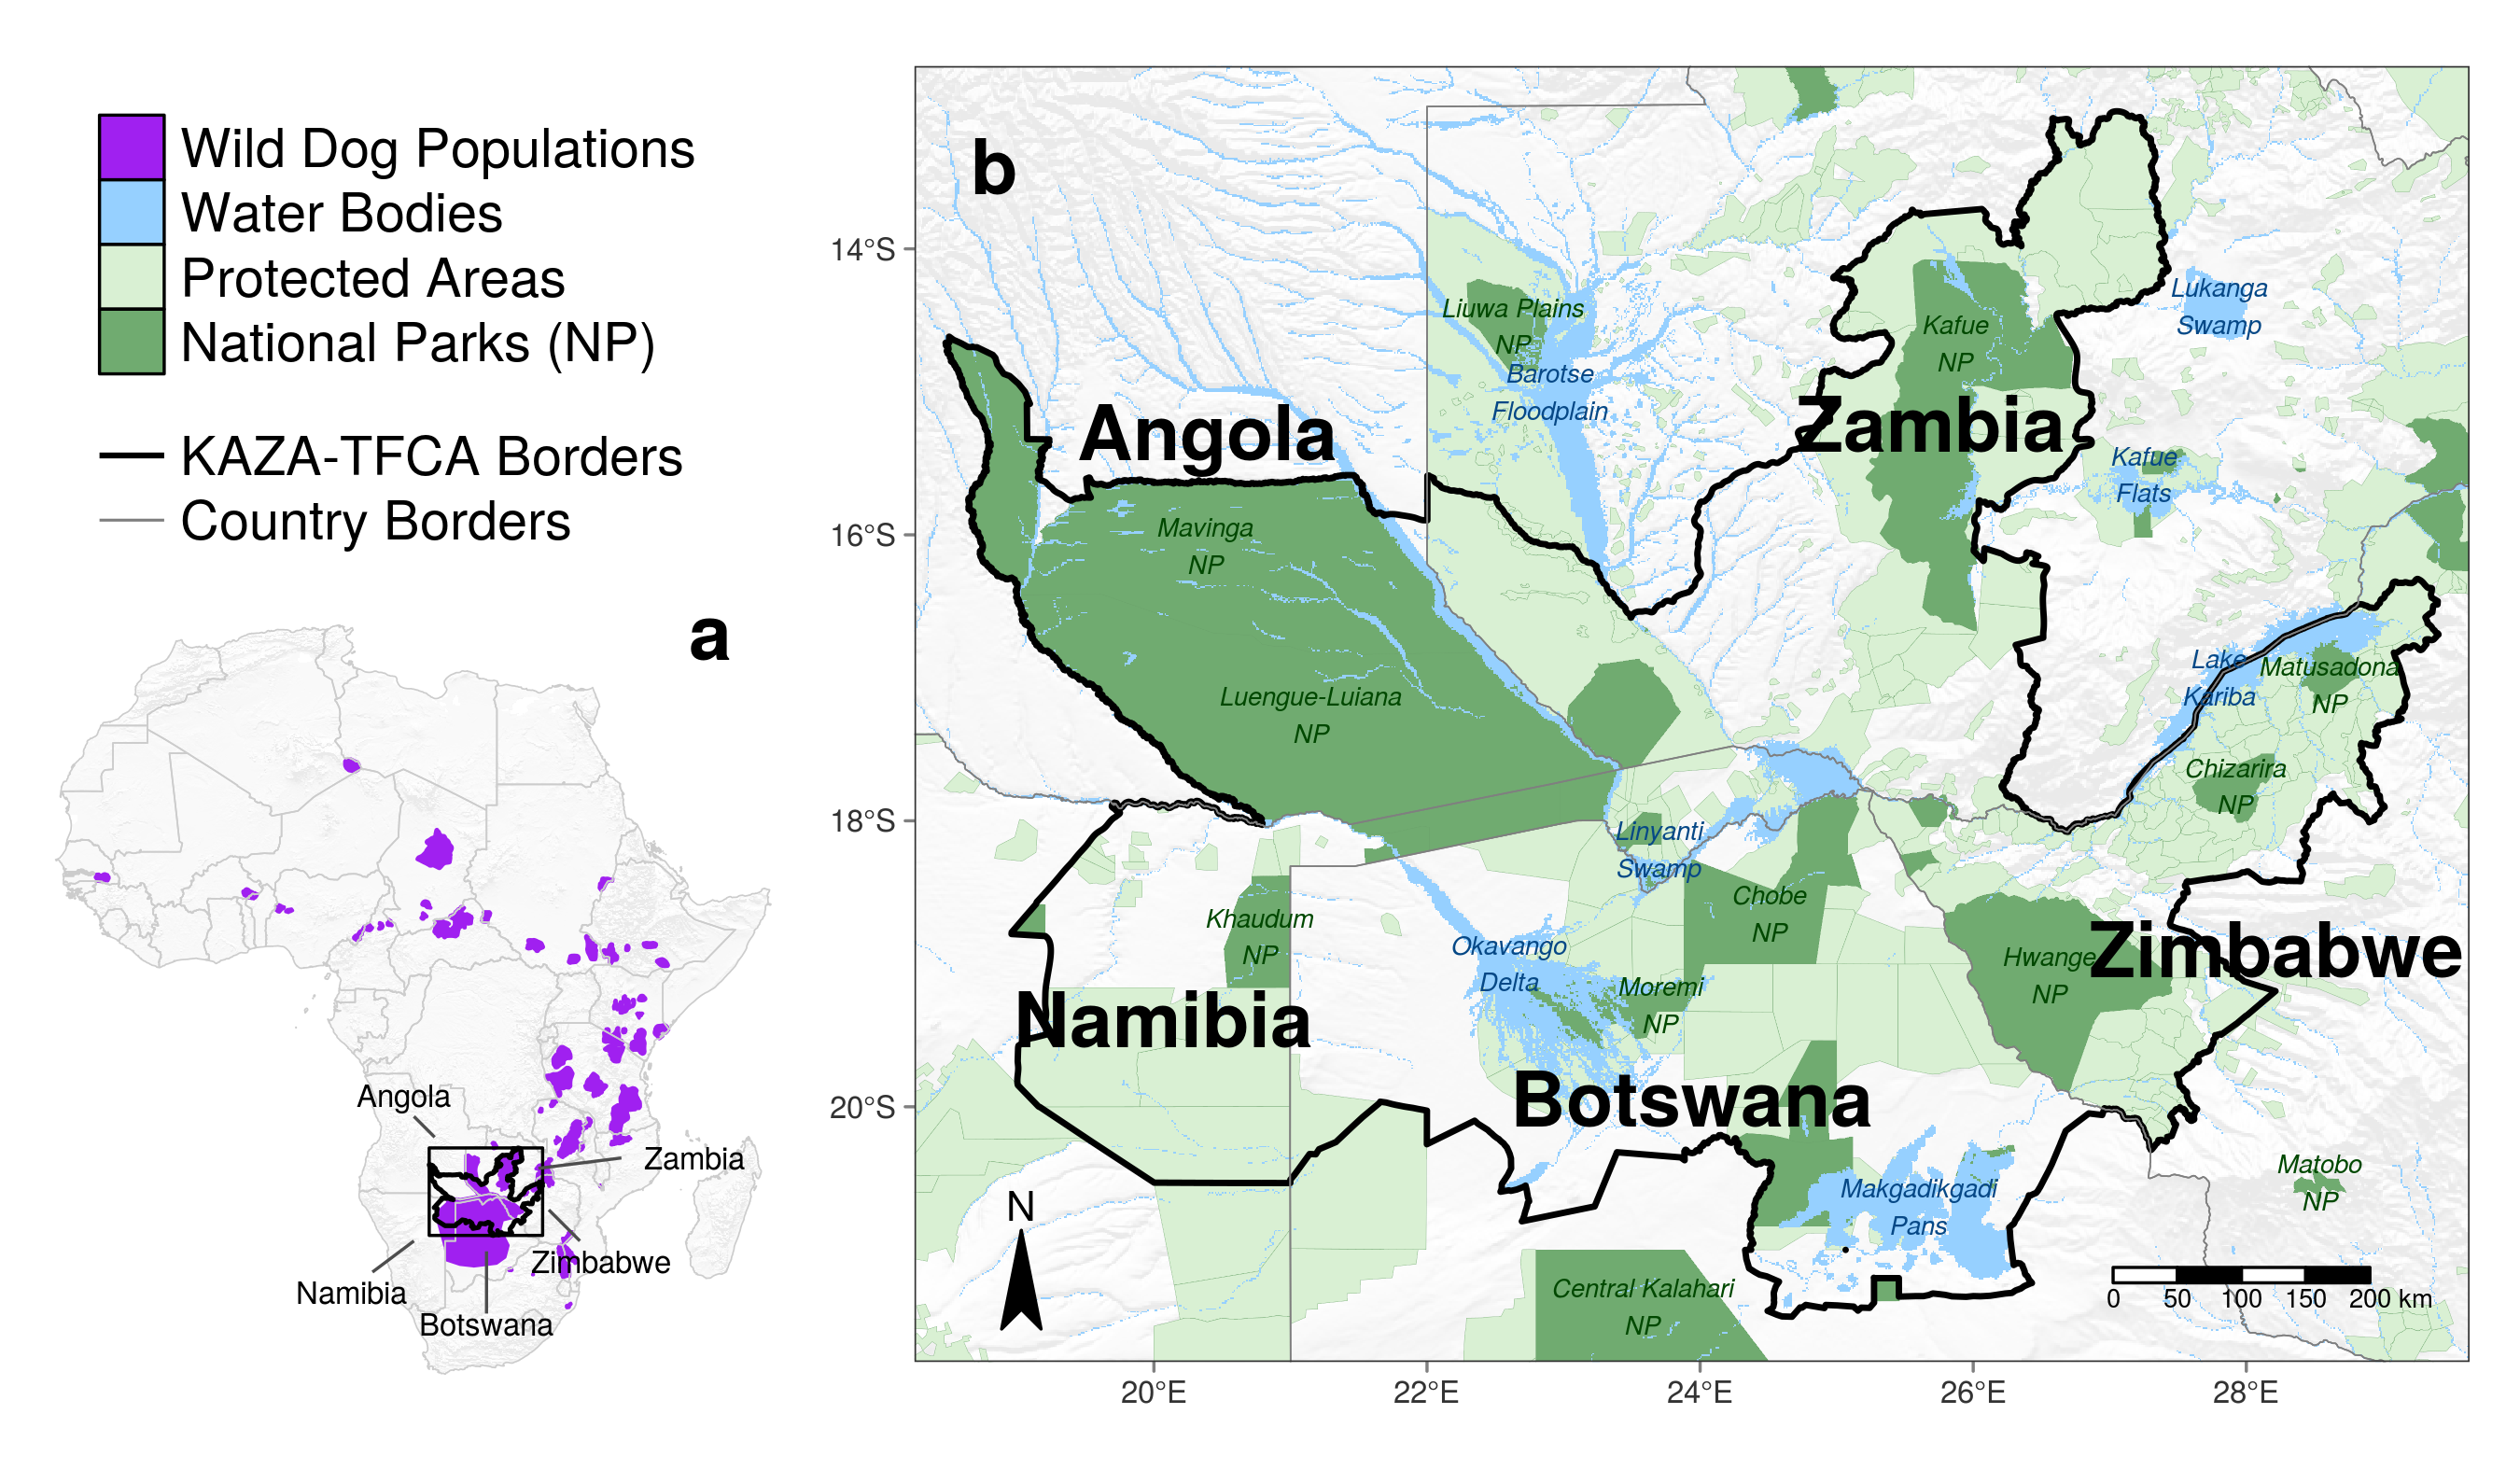
\includegraphics[width = \textwidth]{99_StudyArea.png}
    \caption{(a) The study area of our research was confined by a bounding box
    encompassing the entire KAZA-TFCA, which comprises parts of Angola, Namibia,
    Botswana, Zimbabwe, and Zambia. (b) The KAZA-TFCA represents the world's
    largest terrestrial conservation area and covers a total of 520'000
    km\textsuperscript{2}. It will connect or reconnect multiple already
    existing national parks and protected areas (green polygons) that are
    distributed across its extent. The African wild dog dispersal data
    considered in this study was collected on free-ranging individuals departing
    from the Moremi National Park in northern Botswana (since game reserves in
    Botswana serve the same purpose as national parks, we refer to them as
    national parks for simplicity).}
    \label{StudyArea}
  \end{center}
\end{figure}

\subsection{GPS Relocation Data}
Between 2011 and 2019, we collected GPS relocation data from dispersing wild
dogs in a free-ranging wild dog population inhabiting the Moremi National Park
in northern Botswana. We identified potential dispersers based on age, number of
same‐sex siblings, pack size, and presence of unrelated opposite-sex individuals
in the pack \citep{McNutt.1996, Behr.2020}. We immobilized individuals using a
cocktail of Ketamine/Xylazine/Atropine \citep{Osofsky.1996, Cozzi.2020},
injected with a dart, fired from a CO\textsubscript{2}-pressurized gun
(\textit{DAN-Inject, Denmark}). Anesthesia protocols were approved by the
Ministry of Environment, Natural Resources Conservation and Tourism of Botswana
(permit EWT 8/36/4 XXXVI). After immobilization, individuals were fitted with
GPS/Satellite radio collars (\textit{Vertex Lite; Vectronic Aerospace GmbH,
Berlin}) that included an automated drop-off mechanism. Handling and collaring
of all individuals was carried out and supervised by a Botswana-registered
wildlife veterinarian. All of the immobilized individuals usually rejoined their
pack within one hour after the procedure. Out of all collared individuals, 16
individuals eventually dispersed in separate same-sex coalitions and their
trajectories were successfully recorded (7 female and 9 male coalitions).

During dispersal, collars were programmed to record a GPS fix every 4 hours.
Collected relocations were regularly transmitted over the Iridium satellite
system, which allowed remote tracking of individuals, even if they left the main
study area and crossed international borders. To distinguish between periods of
residency and dispersal, we applied the net-squared displacement metric to the
observed movement data. This metric measures the squared Euclidean distance of a
collared individual to a reference point \citep{Borger.2012}. As a reference
point, we used the center of each disperser's natal home range, such that
dispersal was deemed to have started when an individual left its natal home
range and ended once individuals became sedentary again. For the purpose of this
study, we discarded all data that was collected during residency and only
retained movement data during dispersal. Previous research suggests that females
and males behave similarly during dispersal \citep{Woodroffe.2019, Cozzi.2020},
so we did not distinguish between sexes in our analyses. Ultimately, we
converted the collected GPS coordinates to steps, where each step represented
the straight-line distance traveled by and individual between two consecutive
GPS relocations \citep{Turchin.1998}.

\subsection{Covariates}
We represented the physical landscape in the study area using a set of habitat
covariates rendering water-cover, distance to water, tree-cover, and
shrub/grassland-cover. Because water cover greatly changes within and between
years around the Okavango Delta, we applied a remote sensing technique that
allowed us to generate frequently updated water cover layers and corresponding
distance to water layers (see \citealp{Wolski.2017} and \citealp{Hofmann.2021}).
Hence, the obtained layers temporally aligned with our dispersal events.
Furthermore, we computed a proxy for human influence, depicting anthropogenic
pressures stemming from human-density, agricultural sites, and roads. We
coarsened or interpolated all layers to a target resolution of 250 m by 250 m
and cropped them to the extent of the KAZA-TFCA. Further details on the sources
and preparation of each habitat covariate are given in \cite{Hofmann.2020}.

Besides habitat covariates, we also computed movement metrics that we used as
movement covariates in our models. Movement metrics were calculated for each
step and included the step length (\textsf{sl}), its natural logarithm
(\textsf{log(sl)}), and the cosine of the relative turning angle
(\textsf{cos(ta)}). Because wild dogs follow a diurnal activity pattern, we also
coded a binary variable (\textsf{LowActivity}) indicating whether a step was
realized during low activity (17:00 to 07:00 local time) or high activity (09:00
to 17:00 local time). We conducted all cleaning and analysis, as well as all
simulations using the statistical software {\tt R}, version 3.6.6
\citep{R.2019}. The corresponding {\tt R}-scripts are provided on Github.

\subsection{Movement Model}
We used integrated step selection functions (iSSF) to parametrize a mechanistic
movement model of dispersing wild dogs. In contrast to regular step selection
functions, \textit{integrated} step selection functions allow simultaneous
inference on movement and habitat preferences of the studied animal, and on
potential interactions between habitat and movement preferences. In result, the
method produces less biased selection estimates and allows to treat the
resulting model as a fully mechanistic movement model based on which movement
can be simulated. To conduct iSSF analysis, we paired each observed step with 24
random steps, alltogether forming a stratum that received a unique identifier.
Each of the 24 random steps served as pseudeo-absence and resembled a potential
alternative that the animal could have realized but decided not to. We generated
random steps by sampling random turning angles from a uniform distribution
(\(-\pi, +\pi\)) and step lengths from a gamma distirbution that was fitted to
observed steps (scale = 6'308, shape = 0.37). While the number of random steps
is inversely proportional to the sampling error \citep{Avgar.2016}, a
preliminary analysis revealed only minor differences in model performance when
sampling additional random steps, hence we deemed 24 random steps to be
sufficient. Along each step, we extracted and averaged spatial covariates using
the {\tt velox} package and we calculated the movement metrics \textsf{sl},
\textsf{log(sl)}, and \textsf{cos(ta)}. To facilitate model convergence, we
standardized all continuous covariates to a mean of zero and a standard
deviation of one. Since correlation among covariates was low (\(|r| > 0.6\);
\citealp{Latham.2011}), we retained all of them for modeling.

To compare realized steps (scored 1) to random steps (scored 2), we assumed that
animals assigned a selection score \(w(x)\) to each step. The score depended on
the step's covariates \(X\), as well as the animals preferences \(\beta\)
towards these covariates. The probability of a step being realized was then
contingent on the step's selection score, as well as on the selection scores of
all other step in the same stratum. To estimate the preferences of interest, we
fitted conditional logistic regression models in the r-package {\tt glmmTMB}
following the method proposed by \citep{Muff.2020}. This approach enables to fit
random slopes in addition to random intercepts. Here, we used animal IDs as
random effect and modelled random slopes for each covariate. To apply the
``poisson trick'', we fixed the random intercept variance at an arbitrary high
value of 10\textsuperscript{6} \citep{Muff.2020}.

The structure of our movement model was based on a habitat selection model for
dispersing wild dogs presented in \cite{Hofmann.2021}. In the original model, no
interactions between the habitat and movement covariates were considered, so we
slightly expanded this base model by proposing interactions between movement and
habitat covariates. More specifically, we started with the base model and
incrementally increased model complexity by adding all possible two-way
interactions between habitat covariates and movement covariates. For instance,
for the covariate \textsf{water}, we proposed the interactions
\textsf{Water:log(sl)}, \textsf{Water:log(sl)}, and \textsf{Water:cos(ta)}.
Besides those combinations, we also proposed the interactions
\textsf{sl:cos(ta)} and \textsf{log(sl):cos(ta)} to account for a correlation
between turning angles and step lengths, as well as the interactions
\textsf{sl:LowActivity} and \textsf{log(sl):LowActivity} to account for the fact
that step lengths may differ due to wild dogs' diurnal activity pattern. To
compare competing models and assess the most parsimonious movement model, we ran
stepwise forward model selection based on Akaike's Information Criterion (AIC,
\citealp{Burnham.2002}) and computed model weights.

We validated the predictive power of the selected movement model using a k-fold
cross-validation procedure for case-control studies presented in
\cite{Fortin.2009}. We randomly split the input data into training and testing
data with an 80:20 ratio. Using the training data we parametrized a movement
model based on which we predicted selection scores \(w(x)\) for all steps in the
test data. Within each stratum we then assigned ranks 1-25 to each step based on
predicted selection scores such that rank 1 was given to the step with the
highest score \(w(x)\). Across all strata we determined the realized step's rank
and calculated rank frequencies for realized steps. Finally, we computed
Spearman's rank correlation between ranks and associated frequencies \(r_{s,
realized}\). We replicated the entire procedure 100 times and computed the mean
correlation coefficient (\(\bar{r}_{s, realized}\)), as well as its 95\%
confidence interval across all replicates. For comparison, we repeated the same
procedure 100 times assuming random preferences. Random preferences were
implemented by discarding the realized step from all strata and identifying the
rank of a random step in each stratum. Again, we calculated Spearman's rank
correlation coefficient (\(r_{s, random}\)), its mean across repetitions
(\(\bar{r}_{s, random}\)), and its 95\% confidence interval. This validation
proofs a significant prediction in case the confidence intervals of
\(\bar{r}_{s, realized}\) and \(\bar{r}_{s, random}\) do not overlap.

\subsection{Dispersal Simulation}
We used the most parsimonious movement model to simulate a total of 80'000
dispersing wild dogs moving across the KAZA-TFCA. The simulation resembled an
inverted iSSF and was set up as follows. (1) We sampled a source point at which
a disperser was initiated. We assumed a random initial orientation of the animal
in order to permit calculation of relative turning angles. (2) We generated a
set of 25 random steps by sampling turning angles from a uniform distribution
(\(-\pi, +\pi\)) and step lengths from the fitted gamma distribution. In line
with our training data, each step resembled the straight line movement realized
within 4 hours. To prevent the sampling of unreasonably large steps, we capped
sampled step lengths to a maximum of 35 km, which corresponds to the farthest
distance ever traveled within 4 hours by our dispersers. (3) Along each random
step, we extracted habitat covariates and calculated movement covariates. (4) We
applied the parameterized movement model to predict the selection score \(w(x)\)
for each of the proposed steps and translated selection scores into
probabilities by applying \Cref{EQ2}. (5) We sampled one of the random steps
based on predicted probabilities and used it to determine the animal's new
position. We then repeated steps (2) to (5) until 2'000 steps were realized.

Because some simulated dispersers would inevitably approach a map boundary, some
of the proposed random steps may leave the study area, such that covariates
could be extracted and no selection score could be calculated. To mitigate the
influence of such edge effects, we followed \citep{Koen.2010} and artificially
expanded all covariate layers by adding a 100 km buffer zone within which we
randomized covariate values by resampling values from the observed covariate
layers. This allowed simulated dispersers to leave and reenter the study area
through this buffer zone. Nevertheless, if a disperser approached this outer
boundary and one of the proposed random steps left the buffer, we resampled
transgressing steps until they fully lied within the buffer zone, thereby
forcing dispersers to bounce off the outer boundary. The simulation was mainly
coded in the programming language {\tt R}, yet a few helper functions were
written in {\tt C++} and imported into {\tt R} using the {\tt Rcpp} package
\citep{Eddelbuettel.2011, Eddelbuettel.2013}.

\subsection{Source Points}
To initiate virtual dispersers at biologically meaningful source points, we
randomly placed source points within contiguous protected areas larger \(>\) 700
km\textsuperscript{2} (\Cref{SourcePoints} (a)). This conforms to the average
home range requirement of resident wild dogs \citep{Pomilia.2015} and allowed us
to remove areas too small to host viable wild dog populations. By distributing
source points randomly, the number of source points per km\textsuperscript{2}
within protected areas was approximately equal across our study area. Across all
protected areas, we distributed 50'000 source points, each representing the
starting point of a single dispersal trajectory. To render potential immigrants
into the study system, we placed additional 30'000 source points inside the
buffer zone around the main study area (\Cref{SourcePoints} (b)).

\begin{figure}[htbp]
  \begin{center}
    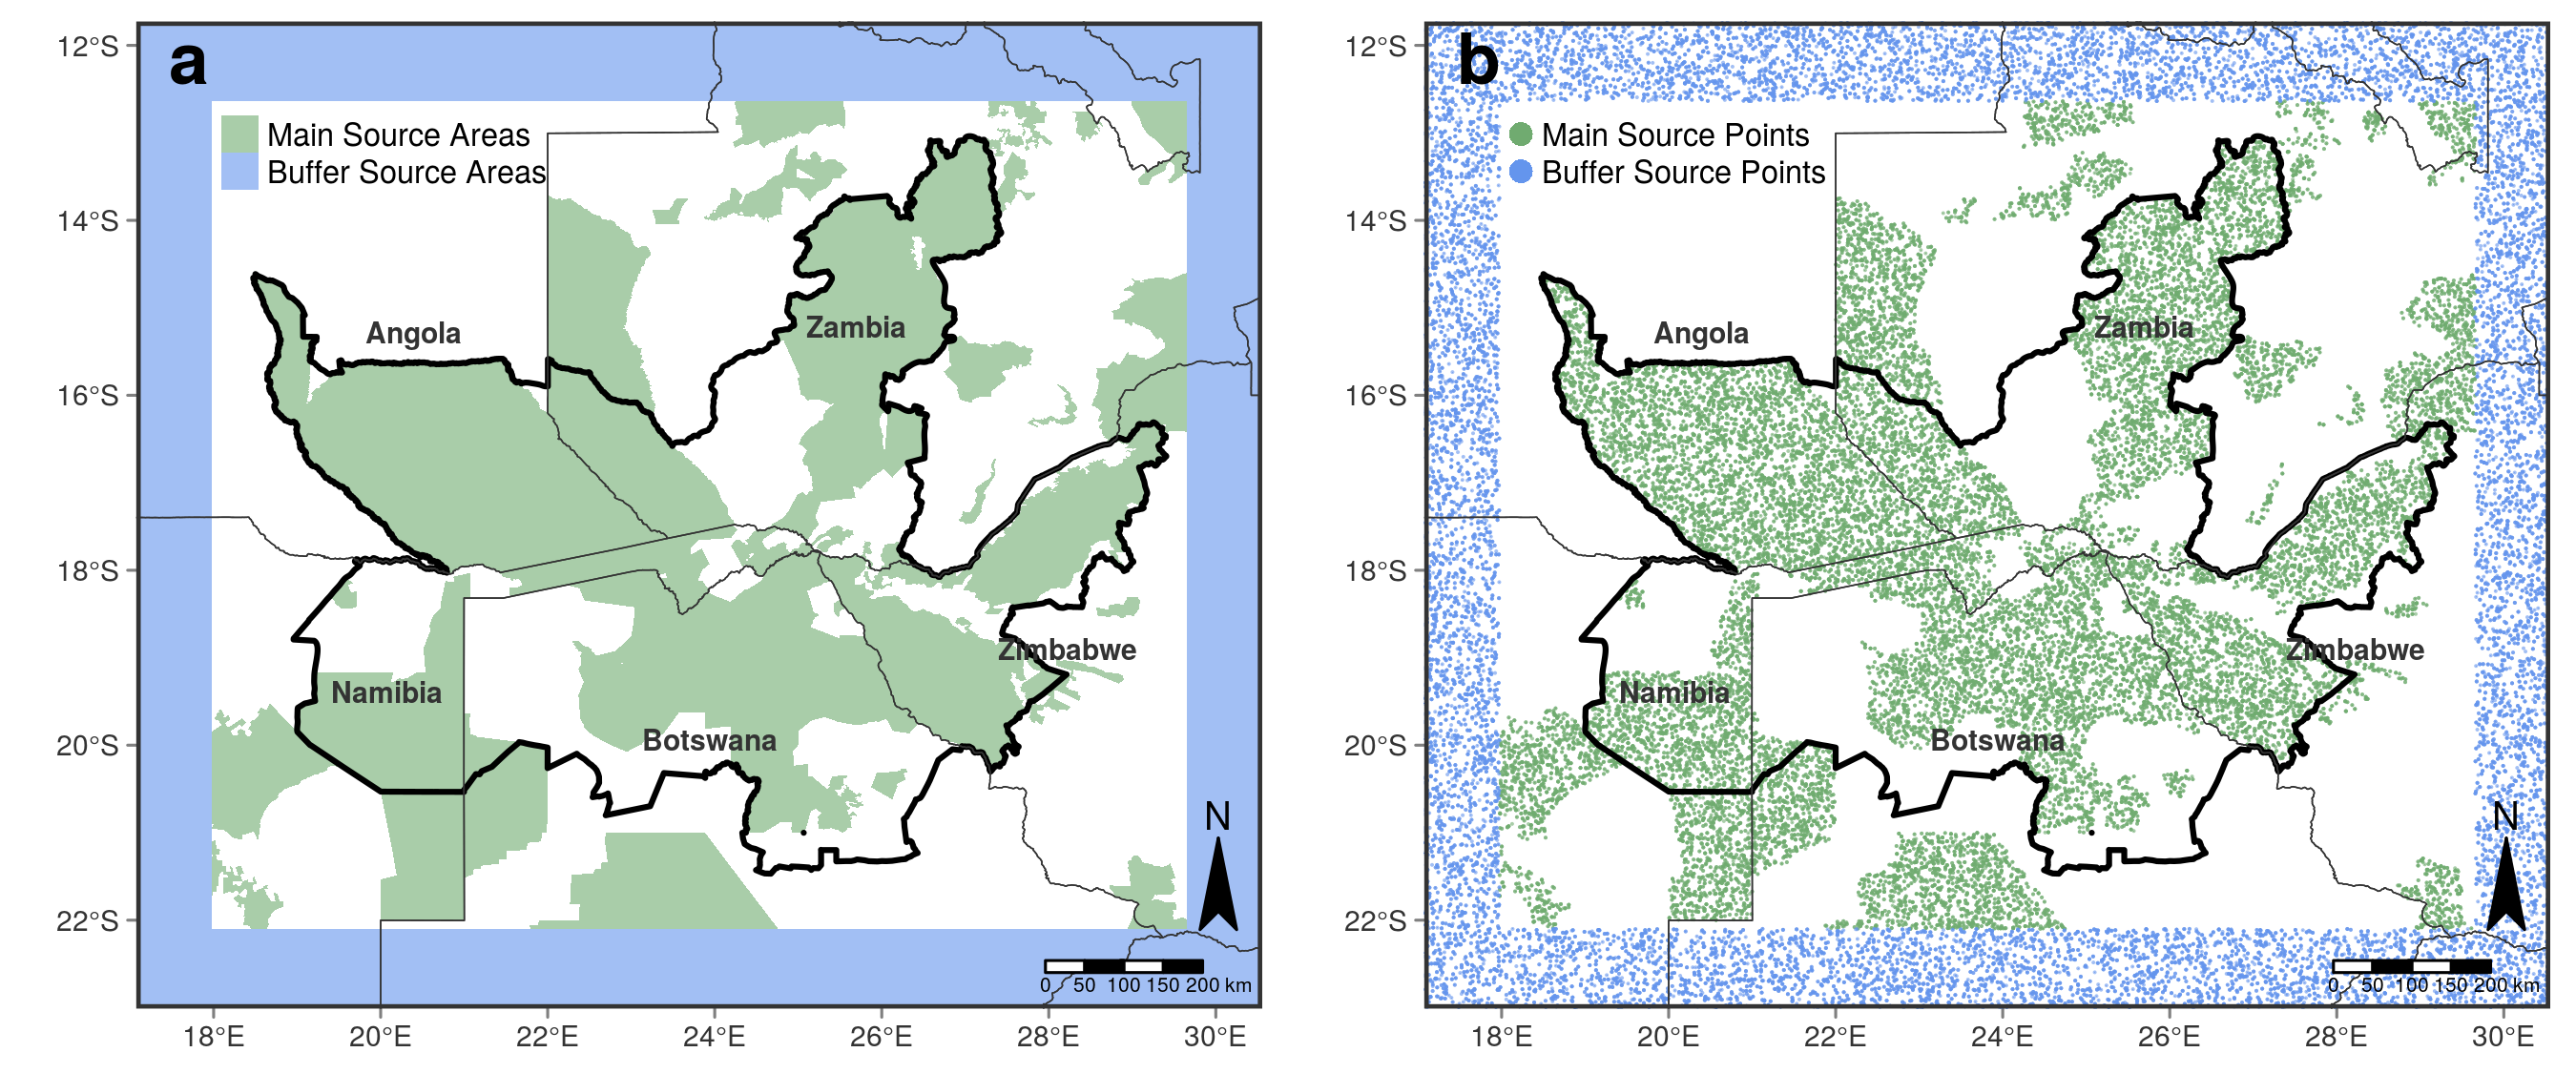
\includegraphics[width = \textwidth]{99_SourceAreas.png}
    \caption{(a) Illustration of an artificially expanded covariate layer (water
    cover). We expanded the layer by adding a 100 km buffer (light blue) which
    we filled with values sampled from the original layer. (b) Different source
    areas from which we released virtual dispersers. We initiated 50'000
    dispersers within the main study area (green) and another 30'000 dispersers
    within a virtual buffer (blue).}
    \label{SourcePoints}
  \end{center}
\end{figure}

\subsection{Heatmaps}
To identify dispersal hotspots across our study area, we rasterized all
simulated trajectories and created a heatmap indicating the absolute frequency
at which each raster-cell in the study area was visited by our virtual
dispersers. If the same trajectory crossed a raster-cell twice, it was only
counted once. That is, we did not consider revisits, thereby mitigating biases
arising from individuals that were trapped in a certain locations and moved
around in circles. We achieved high performance rasterization of all simulated
trajectories using the R-package {\tt terra} \citep{Hijmans.2020}. While one
could easily subset the data to visualize heatmaps assuming different dispersal
durations, we retained all 2'000 simulated steps to create a single heatmap.

% To examine if and how ``heat'' changes in response to changes in the location of
% source points and the number of simulated steps, we followed a 2 x 6 design and
% created heatmaps for both point sampling regines, as well as for 68, 125, 250,
% 500, 1000, and 2000 dispersal steps. We quantified the similarity of the
% resulting 12 heatmaps to the permeability and least-cost corridor maps presented
% in (Hofmann ...) we used Bhattacharyya's affinity. Bhattacharyya's affinity
% ranges from zero (complete separation) to one (perfect match) and has earlier
% been proposed to compare the overlap of utilisation distributions (Fieberg).


\subsection{Network Analysis I}
To pinpoint areas that are of high relevance for connecting remote regions in
our study area, we adopted a network view on the simulated trajecotries and
computed the betweenness metric. More specifically, we overlaid the study area
(including the buffer) with a with a raster that had a cell size of 5 x 5 km,
where each raster-cell represented a node in the final network. We then used the
simulated trajectories to determine all transitions occurring from one cell to
another, as well as the frequency at which these transitions occurred. This
resulted in an edge-list that we translated into a weighted network using the
r-package {\tt igraph}. Because {\tt igraph} handles the weights \(\omega\) as
costs, we inverted the traversal frequency at each cell by applying \(\omega =
\frac{\sum_i^n{Traversal Frequency_i}/n}{Traversal Frequency_i}\). Finally, we
calculated the betweenness metric for each node in the final network. This
metric indicates how often a specific raster-cell lies on a shortest path
between two other raster-cells and is therefore a useful metric to detect
movement corridors \citep{BastilleRousseau.2018}.

\subsection{Network Analysis II}
Besides this, we also adopted an alternative network view and identified the
frequency at which dispersers originating from one national park successfully
moved into an other national park. We achieved this by looking at each pairwise
combination of national parks and determining the relative number of
trajectories that originated in one national park and had at least one
subsequent coordinate laying in the other national park. This allowed us to
determine the average duration it took a simulated disperser to move from one
national park to another, and to point out combinations of national parks
between no links were observed.

\section{Results}
\subsection{Movement Model}
Compared to the base model reported in \citep{Hofmann.2021}, our most
parsimonious movement model included several additional interactions between
habitat and movement covariates (\Cref{MovementModel} and
\Cref{MovementModelNumbers}). Although multiple models received an AIC weight
above zero (T1 in Appendix S1), we only consiered results from the  ``best''
model for further analyses. Since all models with positive AIC weight contained
similar covariates, this decision only marginally influenced subsequent results.
Results from the selected model are given in \Cref{MovementModelNumbers} and
illustrated in \Cref{MovementModel} (a). Additional plots to ease with the
interpretation of the model are provided in Appendix XX.

When holding constant for movement behavior, we find that dispersing wild dogs
avoid water, but prefer its proximity. Dispersers also avoid densely forested
woodlands, yet prefer open shrublands or grasslands. Finally, dispersers avoid
moving through landscapes that are influenced by humans.

When looking at the movement kernel, we observe several significant
interactions. However, except for the interaction \textsf{sl:LowActivity},
estimated slopes are relatively flat, suggesting that our initial distributions
for step lengths and turning angles were only marginally biased. For instance,
the positive effect for \textsf{cos(ta)} indicates that observed turning angles
are slightly more directional compared to the turning angles proposed by our
uniform distribution. On the other hand, the strongly significant and negative
interaction \textsf{sl:LowActivity} reveals that our fitted gamma distribution
produced steps lengths that were substantially larger that those realized by the
dispersers during low wild dog activity.

However, we also find a strongly significant and negative interaction between
the step length and main-activity indicator, showing that realized step lengths
tended to be much shorter during periods of activity in comparison to the steps
proposed by our fitted gamma distribution.

Finally, the significant interactions \textsf{cos(ta):HumanInfluence} and
\textsf{cos(ta):DistanceToWater\textsuperscript{2}} indicate that dispersers
move much more tortuous in areas influenced by humans but more directed when
distant to water.

Results from the k-fold cross-validation procedure show that our model
substantially outperforms a random guess, as the confidence intervals of r.. and
r.. do not overlap. Additionally, we find that the rank correlation slightly
improved in comparison to the base model reported in \citep{Hofmann.2021}.

\begin{figure}
  \begin{center}
    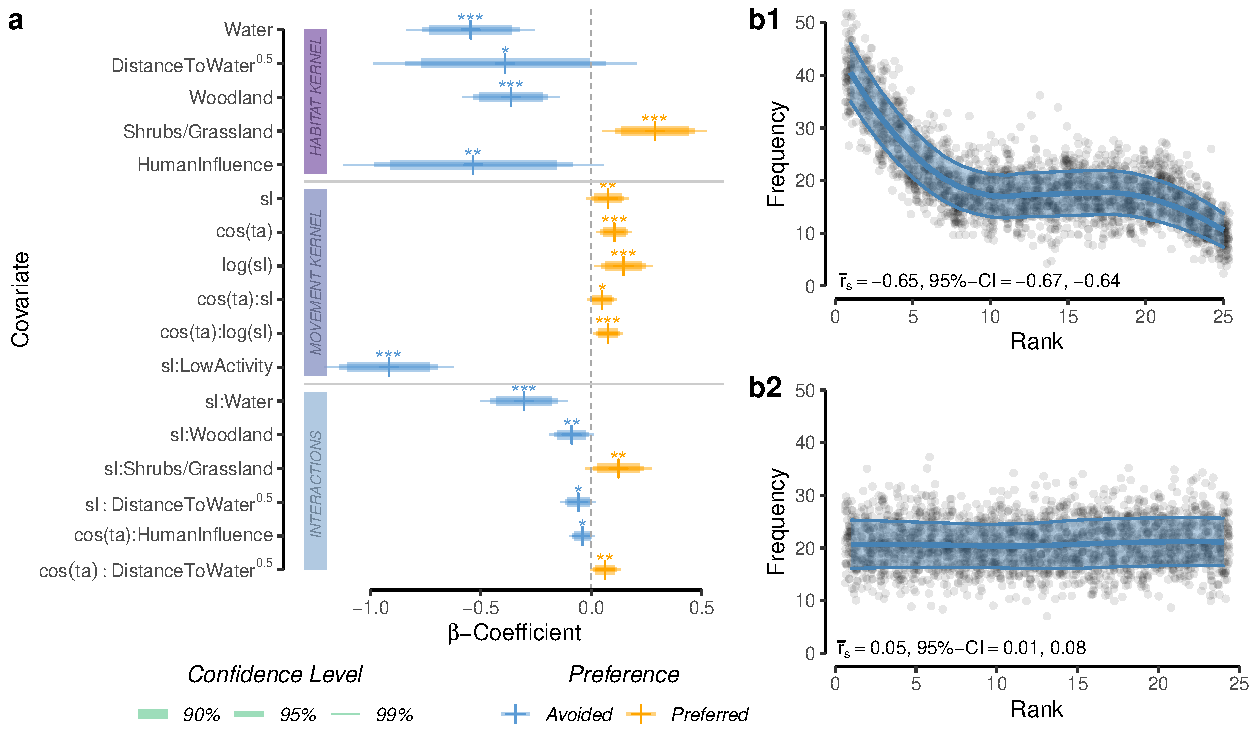
\includegraphics[width=\textwidth]{99_MovementModel}
    \caption{(a) Most parsimonious movement model for dispersing wild dogs. The
    model includes a habitat kernel, a movement kernel, as well as their
    interactions. The orange and blue line segments delineate the 90\%, 95\%,
    and 99\% Confidence-Intervals around the respective \(\beta\) coefficients.
    Significance codes: * \(p < 0.10\), ** \(p < 0.05\), *** \(p < 0.01\). (b)
    Results from the k-fold cross validation procedure. The upper plot shows
    rank frequencies of predicted realized scores according to model predictions
    with known preferences, whereas the lower plot shows rank frequencies when
    assuming random preferences. The blue ribbon shows the prediction interval
    around a loess smoothing regression that we fitted to ease the
    interpretation of the plots.}
    \label{MovementModel}
  \end{center}
\end{figure}

\begin{table}
  \begin{center}
  \caption{Most parsimonious movement model for dispersing wild dogs. The model
  comprises of a movement and habitat kernel, where the movement kernels
  describes preferences with regards to movement behavior, whereas the habitat
  kernel describes preferences with respect to the habitat. Finally, the two
  kernels can interact, such that movement preferences are contingent on habitat
  conditions.}
  \label{MovementModelNumbers}
  \resizebox{\textwidth}{!} {
    \begin{threeparttable}
      \begin{tabular}{llrrrc}
        \toprule
        Kernel & Covariate & Coefficient & SE & pvalue & Significance \\
        \midrule
        \multirow{5}{*}{Habitat Kernel}
         & Water & -0.546 & 0.112 & \(<\) 0.001 & *** \\
         & DistanceToWater \textsuperscript{0.5} & -0.390 & 0.231 & 0.092 & * \\
         & Woodland & -0.364 & 0.086 & \(<\) 0.001 & *** \\
         & Shrubs/Grassland & 0.288 & 0.092 & 0.002 & *** \\
         & HumanInfluence & -0.535 & 0.229 & 0.019 & ** \\
        \hdashline
        \multirow{6}{*}{Movement Kernel}
         & sl & 0.075 & 0.037 & 0.042 & ** \\
         & cos(ta) & 0.105 & 0.031 & 0.001 & *** \\
         & log(sl) & 0.146 & 0.051 & 0.004 & *** \\
         & cos(ta) : sl & 0.049 & 0.026 & 0.064 & * \\
         & cos(ta) : log(sl) & 0.076 & 0.026 & 0.003 & *** \\
         & sl : LowActivity & -0.917 & 0.113 & \(<\) 0.001 & *** \\
        \hdashline
        \multirow{5}{*}{Interaction}
         & sl : Water & -0.305 & 0.076 & \(<\) 0.001 & *** \\
         & sl : Woodland & -0.089 & 0.039 & 0.023 & ** \\
         & sl : Shrubs/Grassland & 0.124 & 0.058 & 0.032 & ** \\
         & sl : DistanceToWater \textsuperscript{0.5} & -0.058 & 0.031 & 0.056 & * \\
         & cos(ta) : HumanInfluence & -0.040 & 0.022 & 0.070 & * \\
         & cos(ta) : DistanceToWater \textsuperscript{0.5} & 0.063 & 0.026 & 0.017 & ** \\
         \bottomrule
      \end{tabular}
       \begin{tablenotes}
         \item \textit{Significance codes: * \(p < 0.10\) \quad ** \(p < 0.05\)
         \quad *** \(p < 0.01\)}
       \end{tablenotes}
    \end{threeparttable}
    }
  \end{center}
\end{table}

\subsection{Dispersal Simulation}
On a machine with an AMD Ryzen 7 2700X processor with 8 x 3.6 GHz and 64 GB of
RAM, a single batch of 1'000 simulated dispersers took roughly 90 minutes to
compute (\(\mu = 88.90\), \(\sigma = 1.87\)). As such, the simulation of all
80'000 dispersers terminated after 120 hours, i.e. five days. However,
comparable computations will be substantially quicker for smaller study areas,
as the covariate extraction from large rasters was computationally the most
expensive task.

On average, step lengths realized by the simulated dispersers (\(\mu = 2'093\)
m, \(\sigma = 3'067\)) were slightly shorter than those by observed dispersers
(\(\mu = 2'326\) m, \(\sigma = 3'323\)). Simultaneously, a slightly smaller
\(cos(ta)\) indicated that simulated dispersers moved with marginally lower
directionality (\(\mu = 0.057\), \(\sigma = 0.071\)) compared to observed
dispersers (\(\mu = 0.078\), \(\sigma = 0.072\)). These differences in step
lengths and turning angles can be attributed to minor disparities between
habitat conditions at the area within which we collected training data and
habitat conditions within the entire study area.

Out of the 50'000 dispersers initiated in protected areas, only 4.5\% eventually
hit a map boundary, highlighting that boundary effects should be neglectable. In
contrast, 78\% of the 30'000 dispersers originating from the buffer zone hit a
map boundary at least once.

\subsection{Heatmaps}
\Cref{Heatmap} depicts the heatmap rendering the traversal frequency at each
pixel of the study area across all simulated individuals and steps. The map
illustrates that large portions of land beyond the borders of the KAZA-TFCA are
only infrequently visited by dispersers (dark blue areas). On the contrary, we
observe that within the KAZA-TFCA extensive regions are regularly visited by
dispersers (bright yellow and red areas). Most notably, the region in northern
Botswana south of the Linyanti swamp glows in rich red and stands out as highly
frequented dispersal hub. Nevertheless, massive water bodies such as the
Okavango Delta, the Makgadikgadi Pan, and the Linyanti swamp, pose considerable
dispersal barriers within and therefore limit realized connectivity the
KAZA-TFCA.

\begin{figure}
  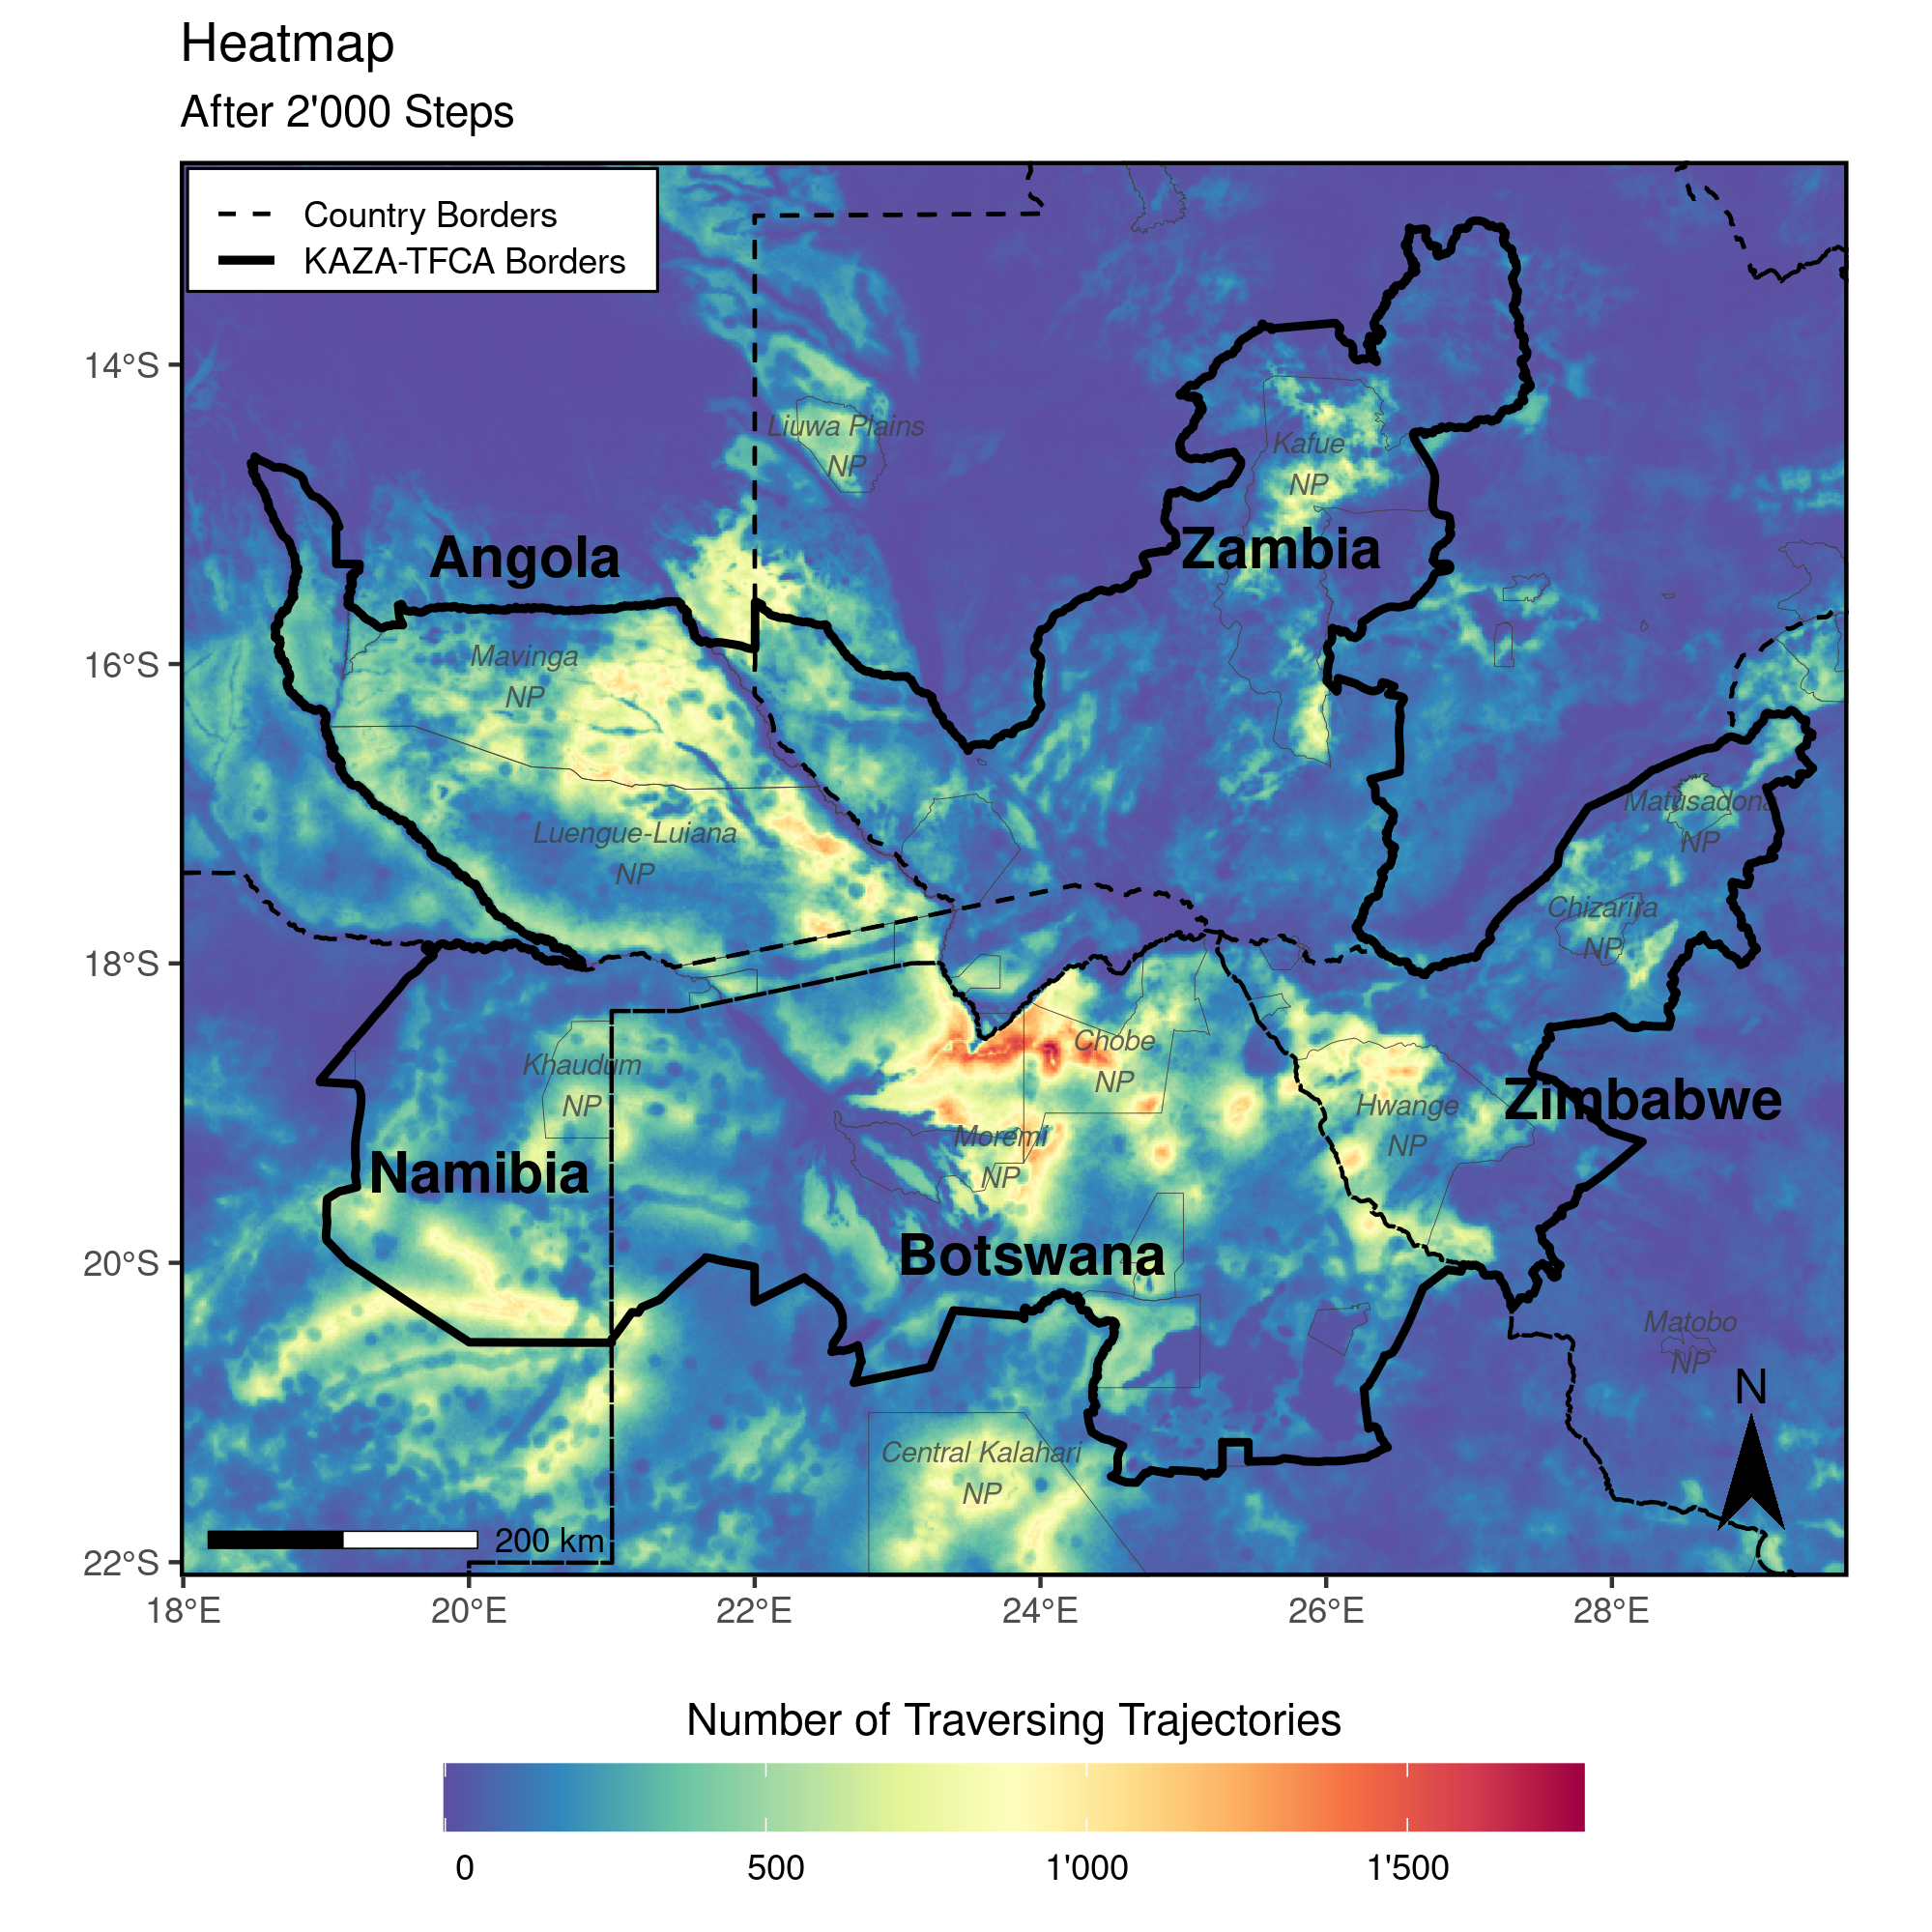
\includegraphics[width=\textwidth]{99_Heatmap.png}
  \caption{}
  \label{Heatmap}
\end{figure}

\subsection{Network Analysis I}
The results of our first network analyses are presented in \Cref{Betweenness}.
In contrast to the heatmap, \Cref{Betweenness} puts much more emphasis on
discrete dispersal corridors. Nonetheless, the dispersal hub in northern
Botswana stands out again and is traversed by a corridor that receives a
comparably high betweenness score. This implies that the region is particularly
crucial for connecting other pixels in the study system and hence represents a
proper dispersal hub. Towards east, the corridor runs through the Chobe National
Park into the Hwange national park, where it branches out and further extends
into the distant Matusadona National Park in Zimbabwe. Northwest of the Linyanty
ecosystem, the same corridor expands into Angola, where it splits and finally
traverses over a long stretch of unprotected area into the Kafue National Park
in Zambia. Several additional corridors with slightly lower betweenness scores
exist, yet most of them run within the boundaries of the KAZA-TFCA. In general,
only few corridors appear to directly link the peripheral regions of the
KAZA-TFCA. For instance, there are no viable dispesal corridors between the
Matusadona National Park in Zimbabwe and the Kafue National Park in Zimbabwe.
Similarly, there are no direct links between the Zimbabwean and Angolan
``spikes'' of the KAZA-TFCA.

\begin{figure}
  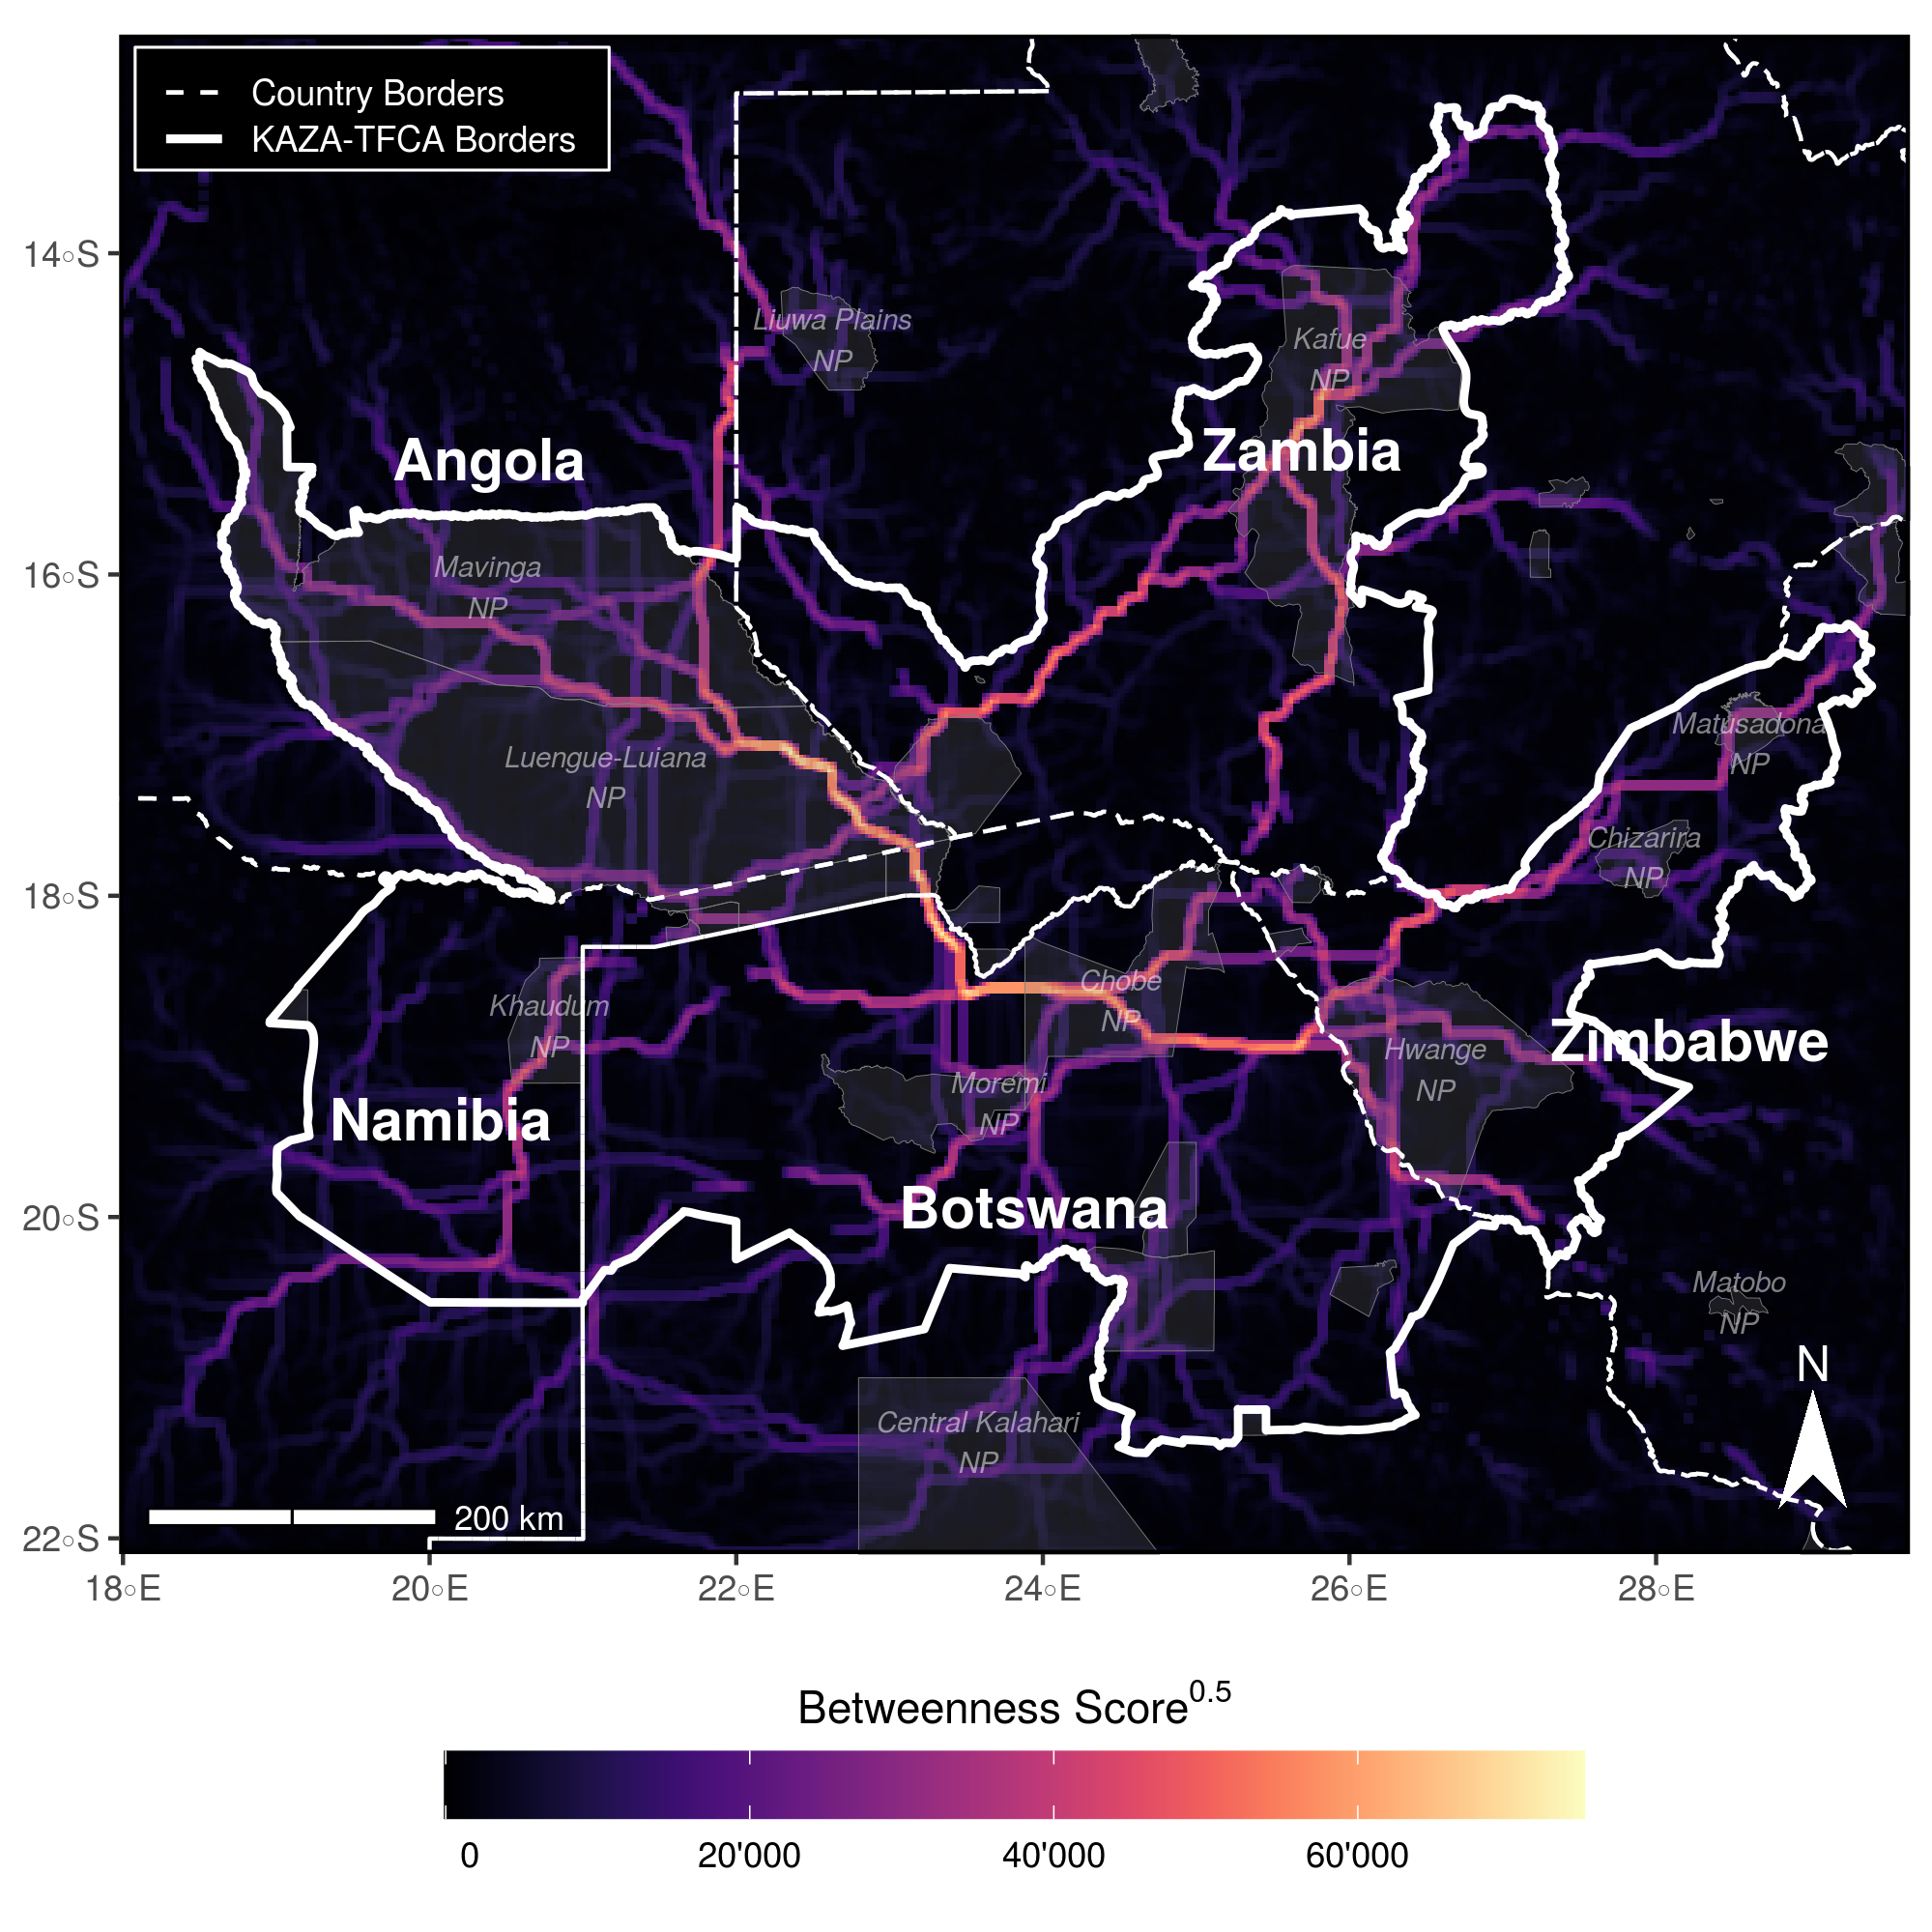
\includegraphics[width=\textwidth]{99_Betweenness.png}
  \caption{Betweenness scores of each raster cell in a raster with 5 x 5 km
  resolution. Betweenness scores were determined based on simulated dispersal
  events. A high betweenness score highlights cells that are exceptionally
  relevant in connecting different regions in the study area. That is, the
  higher the betweenness score, the more often a pixel lies on a shortest path
  between adjacent areas. In this sense the metric can be used to pinpoint
  discrete movement corridors. Note that we square-rooted betweenness scores to
  improve visibility of corrdiors with low scores.}
  \label{Betweenness}
\end{figure}

\subsection{Network Analysis II}
The results from the second network analysis that was focused on connectivity
between national parks are given in \Cref{AreasReached}. The map shows between
which national parks direct links exist and how frequent they are, as well as
the average duration a disperser had to move to realize those links. For
instance, 6.8 \% of the simulated dispersers originating from the Moremi
National Park successfully reached the Chobe National Park and 4.2 \% reached
the Hwange National Park in Zimbabwe. On average, dispersers moved for 623 steps
before arriving at Chobe (SD = 520) and for 1'413 steps before arriving at
Hwange (SD = 371).

\begin{figure}
  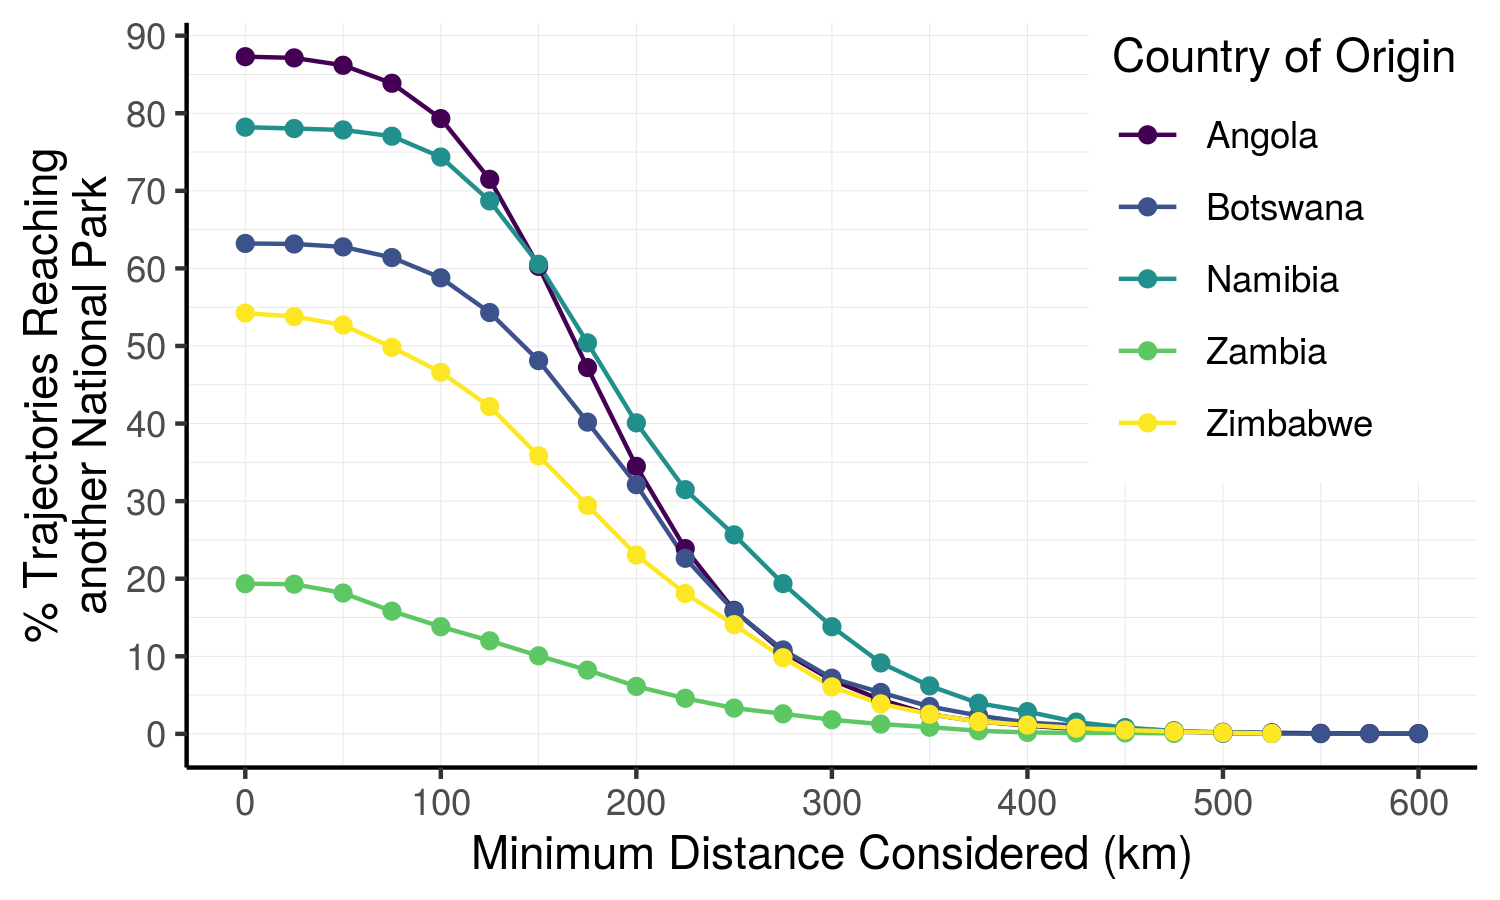
\includegraphics[width=\textwidth]{99_AreasReached.png}
  \caption{Network on simulated dispersal trajectories highlighting the
  connections between national parks (dark green). Yellow bubbles represent the
  center of the different national parks and are sized in relation to the number
  of simulated dispersers originating from each park. Colored arrows between
  national parks illustrate between which national parks the simulated
  dispersers successfully moved and the color of each arrow shows the average
  number of steps that were necessary to realize those connections.
  Additionally, the line thickness indicates the relative number of dispersers
  originating from a national park that realized those connections.}
  \label{AreasReached}
\end{figure}

\section{Discussion}
Our connectivity network further suggests that dispersers from the Okavango
Delta more likely disperse towards east than west. Indeed, only x out of our y
observed dispersers ever reached the western part of the delta. Only when the
flood retracts a small pathway between the city of Maun and the floodwaters of
the delta emerges and enables dispersers to move towards the detal's western
part.

All of our findings are well in line with our previous work, where we have
highlighted dispersal corridors for wild dogs using least-cost approaches. This
suggests that qualitative results are quite insensitive to the exact
methodological approach. Still, we believe that a simulation based approach
offers possibilities for much richer inferences compared to traditional
approaches. This is largely due to the fact that proper movement trajectories
are generated that can be analysed \textit{as if} they were generated by real
dispersers. This is of course contingent on the assumption that underlying
models are adequately representing movement behavior of the focal species and
calls for further methods to validate the predictive power of such simulations.

While the segment running into Kafue receives a high betweenness score, it was
actually only rarely traversed by our simulated dispersers, as can be seen from
the dark colors in this region in \Cref{Heatmap}. It is therefore worth noting
that the betweenness metric highlights crucial bottlenecks that are relevant for
connecting remote regions, yet does not directly yield information about the
absolute frequency at which these bottlenecks are used.

We have previously attributed the weak significance of distance to water to the
fact that we did not control for the presence or absence of conspecifics. We
stick to this reasoning as our expanded model still shows a rather large
uncertainty around the respective beta coefficients. To better gauge the
imporance and influence of this covariate, future studies will need to control
for inter- and intra-speficic interactions that may explain why and when
dispersers are attracted to or afraid of waterbodies.

For our simulations, we represented the Okavango Delta statically and assumed a
relatively extended flood. This resulted in a quasi-barrier, formed by the
Okavango-Delta and the adjacent city of Maun, which was rarely traversed by
simulated individuals. Out of the 499 dispersers initiated inside the Moremi
National Park, only 101 managed to reach the south-western section of the Delta,
whereas 284 eventually reached the equally distant Linyanti swamp. In this
regard, the heatmap presented in \Cref{Heatmap} may be most representative of
the period shortly after the wet-season, when floodlevels in the Delta are at
their maximum. During the dry season, however, the flood considerably retracts
and potentially clears the way for wild dogs dispersing from the Moremi-Game
reserve into the south-western section of the Delta. Future studies could relax
the assumption of a static flood and attempt to update floodlevels as the
dispersers move. This would allow studying how connectivity within the ecosystem
evolves over time as the flood climaxes and retracts again. In fact, one of the
major advantages of such simulation based approaches is that a dynamic
environment can be rendered, as time is explicit in these models
\citep{Zeller.2020}. This contrasts with traditional modelling approaches such
least-cost analysis or circuit theory, where the temporal dimension cannot be
made explicit. An explicit view on time also directly translates in insights on
the duration required by dispersers to move between distinct patches such as
national parks or spatially segregated subpopulations.

Comparable simulations that are based on empirical data are also a fundamental
component for spatially realistic population models in which dispersal is
rendered more realistically and does not merely depend on the distance between
habitat patches.

We did not model mortality during dispersal in our simulations. This was a
simplifying assumption and only inaccurately reflects dispersal in reality. It
is well known that wild dogs often die during dispersal in result of deadly
encounters with other predators, but also due to road kills and illegal
shootings by humans. In result, mortality during dispersal may limit realized
connectivity, especially in areas that wild dogs are unfamiliar with or in areas
with high potential for human-wildlife conflict \citep{Cozzi.2020}.
Interestingly though, \cite{Behr.2021} have recently demonstrated that mortality
during dispersal is lower compared to residency, suggesting the presence some
fitness benefits to dispering individuals.

In this regard, our approach is rather similar to dispersal kernels, yet it
enables to render directional biases, which are currently difficult to implement
using such methods.

We completely randomized the location of source points within protected areas.
However, in some cases prior knowledge about the density of potential dispersers
is available and can be used to adjust the number of simulated individuals
accordingly. Alternatively, instead of tweaking the number of simulated
individuals, one could assign a weight to each trajectory that depends on the
density of potential dispersers in the source areas. As such, trajectories from
areas with high density would enter the heatmap with above average weigth.

The parametrized movement model could also be manipulated to investigate how
different habitat preferences influence landscape connectivity and to test the
sensitivity of results with respect to the exact preferences of individuals.

One of the major benefits of individual-based simulations is the ability to make
the temporal dimension of movement explicit. This allows to investigate how
connectivity depends on the dispersal duration, something that is not possible
with traditional least-cost or circuit theory methods.

Optimally, one should simulate additional dispersers until the amount of newly
gained information lies beyond a certain threshold, i.e. until some sort of
convergence is achieved. However, due to the myriad of outcomes in movement
behavior, this would often imply countless repetitions for each source points at
each location where dispersal is possibly initiated. This is computationally
infeasible.

Our work suggests that the selection of source points significantly impacts
resulting connectivity networks. Especially when dispersal durations are short,
wrongly placed source points lead to vastly different results. Signer et al.
used estimated utilisation distributions by means of simulated movements. They
used a rather long burn in period prior to alleviate the problem of selecting
meaningful source points. However, this approach only works when individuals
move around a point of attraciton. This is typically not the case when
simulating dispersers, introducing an important trade-off. The researcher can
decide to increase the number of simulated steps, hence reducing the influence
of starting locations, yet this also inevitably increases estimated
connectivity.

In some European countries, the comeback of large predators, such as bears,
lynx, and the wolf, has triggered emotional discussions and raised public
concern \citep{Behr.2017}, particularly in areas with free-roaming livestock
that may be prayed upon by the returned species. In cases were recent locations
of such predators are known, an early warning system based on simulations could
serve to forewarn about potential encounters and and thereby increase public
acceptance of large predators.

\section{Authors' Contributions}
D.D.H., D.M.B., A.O. and G.C. conceived the study and designed methodology;
D.M.B., G.C., and J.W.M. collected the data; D.D.H. and D.M.B. analysed the
data; G.C. and A.O. assisted with modeling; D.D.H., D.M.B., and G.C. wrote the
first draft of the manuscript and all authors contributed to the drafts at
several stages and gave final approval for publication.

\section{Data Availability}
GPS movement data of dispersing coalitions will be made available on dryad at
the time of publication.

\section{Acknowledgements}
We thank the Ministry of Environment and Tourism of Botswana for granting
permission to conduct this research. We thank C. Botes, I. Clavadetscher, and G.
Camenisch for assisting with wild dog immobilizations. We also thank B. Abrahms
for sharing her data of three dispersing wild dogs. Furthermore, we are indebted
to Johannes Signer for assisting with the simulation algorithm. This study was
funded by Basler Stiftung für Biologische Forschung, Claraz Foundation, Idea
Wild, Jacot Foundation, National Geographic Society, Parrotia Stiftung, Stiftung
Temperatio, Wilderness Wildlife Trust Foundation, Forschungkredit der
Universität Zürich, and a Swiss National Science Foundation Grant
(31003A\_182286) to A. Ozgul.

\newpage
\begingroup
\singlespacing
\bibliography{Literatur}
\endgroup

\end{document}
